\chapter{Návrh používateľského rozhrania a štruktúry aplikácie}\label{chap:navrh}
Táto kapitola opisuje vizuálny návrh aplikácie Office Hours: od prvých ručných náčrtov cez prototyp až po návrh štruktúry projektu a možnosti budúceho rozšírenia.

\section{Návrh používateľského rozhrania}\label{sec:navrh-ui}
Cieľom návrhu používateľského rozhrania bolo vytvoriť moderné a predovšetkým intuitívne prostredie, ktoré umožňuje používateľovi rýchlo a bezchybne vykonať požadovanú akciu.

\subsection{Od počiatočných náčrtov k prototypu vo Figme}
Proces návrhu používateľského rozhrania začal sériou iteratívnych konzultácií s vedúcim bakalárskej práce. Prvotná vízia rozmiestnenia kľúčových prvkov – ako sú zoznamy miestností, časové bloky a rezervačné dialógy – bola vytvorená vo forme jednoduchých ručných náčrtov (tzv. wireframes). Tento prístup umožnil rýchlu a flexibilnú validáciu základnej informačnej architektúry.

Následne bol tento overený koncept pretransformovaný do interaktívneho prototypu v grafickom editore Figma. Pri tomto návrhu bol striktne dodržiavaný prístup \uv{Mobile-first}, čo znamená, že aplikácia bola primárne navrhovaná pre malé dotykové obrazovky smartfónov~\cite{mobilefirst}. Tento prístup zaručil, že kľúčové ovládacie prvky (napríklad potvrdzovacie tlačidlá alebo navigácia) sú umiestnené v tzv. zóne pohodlného dosahu palca, zatiaľ čo menej dôležité informácie alebo nadpisy sa nachádzajú v hornej časti obrazovky.

\begin{figure}[t]
    \centering
    \begin{minipage}[t]{0.45\textwidth}
        \centering
        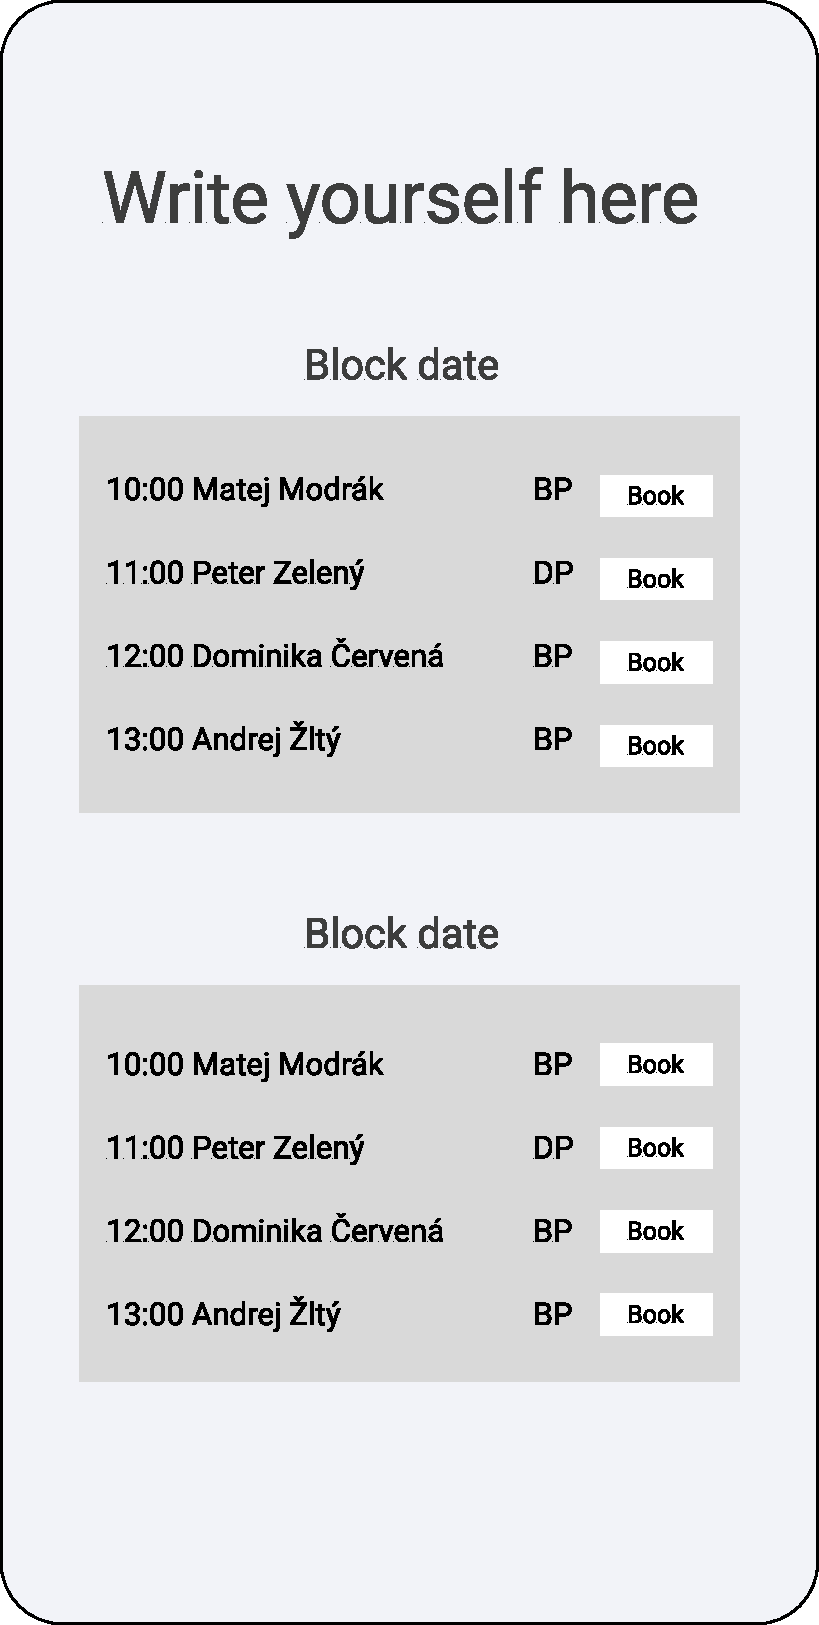
\includegraphics[width=\textwidth]{obrazky-figures/navrh-wireframe-visitor.pdf}
    \end{minipage}
    \hfill
    \begin{minipage}[t]{0.45\textwidth}
        \centering
        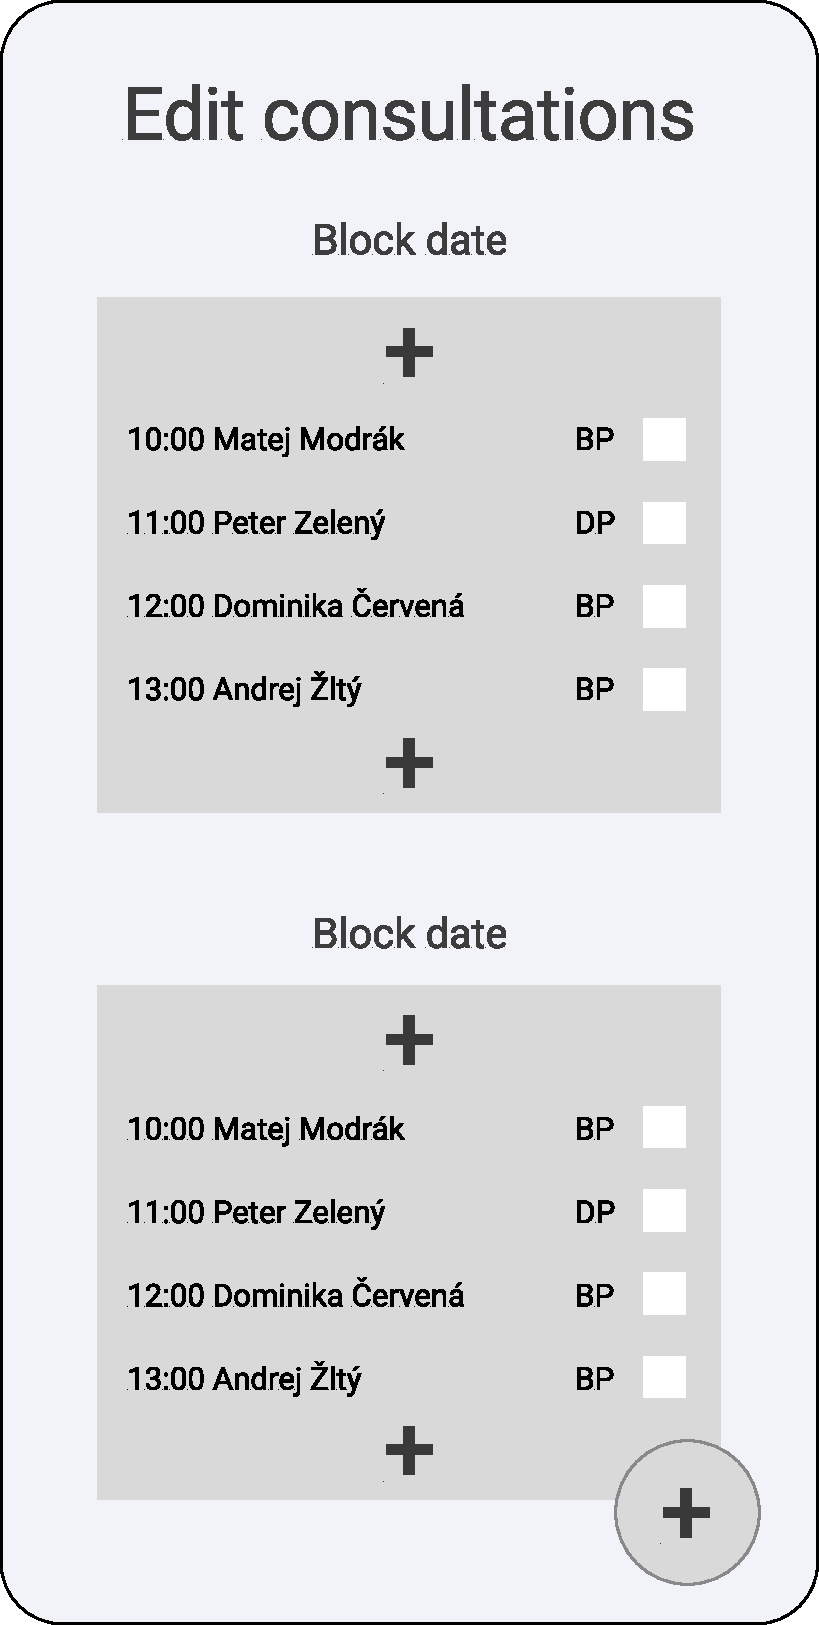
\includegraphics[width=\textwidth]{obrazky-figures/navrh-wireframe-owner.pdf}
    \end{minipage}   
 
    \caption{Wireframy znázorňujúce domovskú obrazovku Návštevníka (naľavo) a Majiteľa (napravo).}   
    \label{fig:wireframes}
\end{figure}



\subsection{Princípy použiteľnosti pre user interface (UI) dizajn}
Návrh aplikácie Office Hours sa riadil heuristikami použiteľnosti (Usability Heuristics) podľa Jakoba Nielsena~\cite{nielsen}.

\begin{itemize}
    \item \textbf{Viditeľnosť stavu systému (Visibility of system status):} Systém by mal používateľa vždy vhodne a včas informovať o tom, čo sa deje. Táto heuristika je implementovaná vizuálnou spätnou väzbou: po odoslaní požiadavky na server sa tlačidlo okamžite zmení na indikátor načítavania, čím sa zabráni viacnásobnému odoslaniu formulára. Rovnako po dokončení každej operácie (napríklad rezervácii slotu) systém zobrazí potvrdzujúcu Toast notifikáciu.

    \item \textbf{Zhoda medzi systémom a skutočným svetom:} Systém by sa mal inšpirovať správaním z reálneho sveta. V aplikácii sa to prejavuje okrem iného prirodzenou fyzikou scrollovania (tzv. rubber-band effect) – keď používateľ dosiahne koniec zoznamu slotov, obrazovka sa prirodzene natiahne a odpruží späť, čím signalizuje používateľovi koniec obsahu.
    
    \item \textbf{Kontrola a sloboda používateľa (User control and freedom):} Používatelia musia mať vždy k dispozícii jasne viditeľné tlačidlo pre núdzový odchod z nežiaduceho stavu. Každá vnorená obrazovka v aplikácii (napríklad detail miestnosti) preto obsahuje výraznú šípku na krok späť v ľavom hornom rohu. Na domovskej obrazovke túto rolu plní vysúvacie \uv{hamburger} menu. Pri deštruktívnych akciách (napríklad zmazanie miestnosti) systém vyžaduje explicitné potvrdenie dialógovým oknom.

    \item \textbf{Konzistencia a štandardy:} Konzistencia umožňuje používateľovi vytvoriť si stabilný mentálny model aplikácie. V Office Hours je uplatňovaná jednotnou terminológiou, vizuálnou štandardizáciou a 4pt grid systémom, ktorého deliteľnosť hodnotami 2, 4 a 8 umožňuje prirodzené škálovanie komponentov~\cite{grid4pt}. Dizajnový systém je striktne obmedzený na 4 veľkosti písma, 2 hrúbky a úzky set farieb.

    \item \textbf{Prevencia chýb (Error prevention):} Aplikácia je navrhnutá tak, aby bolo ťažké urobiť chybu. Napríklad textové polia používajú špecifické typy klávesníc (napríklad email pre e-mailové adresy) a validácia prebieha ešte pred odoslaním na server.

    \item \textbf{Rozpoznanie, nie vybavovanie si (Recognition rather than recall):} Zaťaženie pamäte používateľa sa minimalizuje tým, že sú všetky dôležité akcie a informácie viditeľné. Namiesto toho, aby si používateľ pamätal identifikátory slotov, aplikácia zobrazuje všetky termíny farebne odlíšené (biele = voľné, červené = cudzie, modré = vlastné). Autocomplete pole na obrazovke pripojenia do miestnosti dynamicky dopĺňa názvy ešte počas písania, čím používateľa zbavuje nutnosti pamätať si presný názov miestnosti.
    
    \item \textbf{Flexibilita a efektívnosť používania (Flexibility and efficiency of use):} Systém by mal vyhovovať neskúseným aj pokročilým používateľom. V Office Hours je to implementované viacerými spôsobmi: Majiteľ môže vytvoriť nový blok rýchlym tlačidlom s ikonkou plus priamo na hlavnej obrazovke (bez nutnosti prechádzať menu). Pri vytváraní bloku podporuje výber viacerých dátov naraz (režim „range“ alebo „multiple“). Prepínač medzi rolami (Owner/Visitor) umožňuje rýchlu zmenu kontextu bez prihlasovania a odhlasovania. Pokročilí používatelia môžu využívať funkcie ako kopírovanie celých blokov na iný dátum.
\end{itemize}

\subsection{Aplikácia dizajnových princípov a vizuálna identita}

Farebná paleta využíva neutrálne pozadie, ktoré necháva vyniknúť kľúčové údaje a interaktívne prvky. Primárnou farbou je sýta modrá, používaná výhradne na interaktívne komponenty (tlačidlá, aktívne záložky), aby si používateľ rýchlo vytvoril mentálny model kliknuteľných prvkov. Pre deštruktívne akcie sa používa červená farba.
    
Typografia je navrhnutá tak, aby vytvárala jasnú vizuálnu hierarchiu primárne cez veľkosť a hrúbku písma, nie zmenou farieb. Nadpisy (napríklad názvy miestností) sú výrazné a ľahko skenovateľné, doplnkové informácie sú zobrazené menším písmom a so zníženou nepriehľadnosťou, čo prirodzene vedie oko od najdôležitejších prvkov k detailom.

Výrazným vizuálnym prvkom sú tvary typu squircle, teda zaoblenejšie superelipsy známe z iOS dizajnu. Tieto tvary pôsobia jemnejšie než klasické obdĺžniky s jednoduchým border-radius, čím rozhraniu dodávajú modernejší a priateľskejší charakter.

\section{Návrh jednotlivých častí aplikácie}\label{sec:navrh-casti}
Táto sekcia postupne prechádza návrhom obrazoviek aplikácie Office Hours – od autentifikácie cez pohľad Návštevníka až po rozhranie Majiteľa miestnosti – a opisuje rozhodnutia, ktoré formovali výsledný používateľský tok.

\subsection{Úvodná obrazovka a autentifikácia}
Prvým vizuálnym dojmom aplikácie je splash obrazovka (úvodná dočasná obrazovka, ktorá sa zobrazí pri spustení aplikácie) s logom Office Hours. Počas jej zobrazovania prebehne inicializácia aplikácie.

Po splash obrazovke nasleduje prihlasovacia obrazovka, kde používateľ zadá svoju e-mailovú adresu. Kľúčovým dizajnovým rozhodnutím je, že aplikácia sama rozhodne, čo nasleduje. Používateľ sa tak nemusí rozhodovať medzi možnosťami prihlásenia a registrácie. Ak e-mail nie je evidovaný v systéme, aplikácia ho plynulo presmeruje na registračnú obrazovku s predvyplneným e-mailom, kde doplní meno, priezvisko a účel návštevy. Ak účet už existuje, pokračuje priamo na overenie.

Toto riešenie prináša UX výhodu v podobe zjednodušeného vstupného toku, no zároveň so sebou nesie bezpečnostný kompromis. Rozdielna reakcia aplikácie na registrovaný a neregistrovaný e-mail umožňuje tzv. enumeráciu používateľov – útočník môže systematickým zadávaním e-mailových adries zistiť, ktoré z nich sú v systéme registrované. V kontexte tejto aplikácie, určenej primárne pre akademické prostredie s obmedzeným okruhom používateľov, bolo toto riziko vedome akceptované v prospech jednoduchosti používateľského zážitku. 

V oboch prípadoch nasleduje obrazovka overenia pomocou jednorazového kódu (OTP), ktorý je doručený na zadaný e-mail. Tento krok zabraňuje zneužitiu cudzích e-mailových adries a neoprávnenému zaberaniu miesta v databáze.

\subsection{Pohľad Návštevníka}

\subsubsection*{Úvodná obrazovka a pripojenie do miestnosti}
Po úspešnom prihlásení sa Návštevník, ktorý ešte nie je pripojený do žiadnej miestnosti, ocitne na úvodnej obrazovke. Tá mu zobrazí výzvu na pripojenie sa do prvej miestnosti spolu s priamym odkazom na obrazovku Join Room, čím sa eliminuje zbytočná navigácia.

Na obrazovke Join Room sa nachádza textové pole, ktoré počas písania automaticky dopĺňa názvy dostupných miestností (autocomplete). Používateľ vyberie požadovanú miestnosť zo zoznamu a potvrdí pripojenie.

\subsubsection*{Hlavná obrazovka s miestnosťami, blokmi a slotmi}
Po pripojení do miestnosti sa Návštevník dostane na hlavnú obrazovku konzultácií. V hornej časti obrazovky sa nachádza prepínač miestností (room selector), ktorý umožňuje rýchle prepínanie medzi viacerými miestnosťami v prípade, že sa Návštevník konzultuje u viacerých vyučujúcich. Priamo pod ním je umiestnené odkazové tlačidlo smerujúce na externý link miestnosti. Napríklad na link pre online konzultácie alebo na osobnú stránku vyučujúceho.

Ak v miestnosti zatiaľ neboli vytvorené žiadne bloky, obrazovka zobrazí informatívny text. V opačnom prípade sú zobrazené bloky s ich slotmi. Hlavička každého bloku obsahuje dátum konania a počet dní zostávajúcich do začiatku bloku, čo Návštevníkovi pomáha pri plánovaní. Voliteľne si tu môže aktivovať notifikácie pre daný blok, aby bol upozornený napríklad v prípade uvoľnenia obsadeného slotu.

Samotné sloty sú farebne odlíšené podľa svojho stavu:
\begin{itemize}
    \item \textbf{Biele:} Voľný slot označený ikonkou plus v krúžku, ktorý je možné rezervovať kliknutím na neho.
    \item \textbf{Červené:} Obsadený cudzí slot s textom a ikonkou v utlmenej farbe, ktorá na červenom pozadí vytvára vizuálny dojem neprístupnosti a signalizuje, že slot nie je možné rezervovať.
    \item \textbf{Modré:} Vlastný rezervovaný slot patriaci prihlásenému Návštevníkovi.
\end{itemize}

Pri kliknutí na voľný (biely) slot sa zobrazí vysúvací dialóg (\textit{bottom sheet}), ktorý Návštevníkovi umožní rezerváciu potvrdiť a zároveň ju bližšie špecifikovať, ako je znázornené na obrázku~\ref{fig:slot-dialog}. Dialóg obsahuje predvyplnené textové pole s dôvodom návštevy (\textit{visit purpose}), ktorý si používateľ nastavil v nastaveniach, pričom ho môže pred odoslaním ľubovoľne upraviť. Ďalšou voliteľnou možnosťou je prepínač online/offline konzultácie. Tento prepínač je však dostupný len v prípade, ak Majiteľ daný blok explicitne neoznačil ako online – napríklad z dôvodu choroby alebo iných okolností vynucujúcich dištančnú formu. V takom prípade je online režim pevne nastavený samotným Majiteľom a Návštevník ho nemôže zmeniť. Ak Majiteľ online režim bloku neurčil, Návštevník si môže sám zvoliť, či preferuje konzultáciu prezenčne alebo online.

Na vlastnom (modrom) slote sa nachádza ikonka \textit{X} umožňujúca zrušenie rezervácie a ikonka obrazovky signalizujúca, že konzultácia prebehne online. V tele slotu je zobrazený čas konania a dôvod návštevy (\textit{visit purpose}).

Toto riešenie sa zámerne odlišuje od Google Kalendára analyzovaného v kapitole~\ref{chap:analyza}, kde sú obsadené sloty pre návštevníka úplne skryté. Viditeľnosť všetkých slotov umožňuje Návštevníkovi sledovať aj plné termíny a prípadne si aktivovať upozornenie pre prípad uvoľnenia preferovaného slotu.

Vývoj obrazovky Návštevníka prebiehal iteratívne na základe spätnej väzby. Prvý prototyp (obrázok~\ref{fig:visitor-old}) obsahoval dedikované tlačidlo \textit{Book} pri každom slote a ikonky strážneho psa pre notifikácie, ktoré sa v testovaní ukázali ako príliš komplexné a pre používateľov nejasné. Ikonka online stavu bola taktiež nejednoznačná. Na základe konzultácií s vedúcim práce a spätnej väzby od spolužiakov bol vytvorený druhý prototyp (obrázok~\ref{fig:visitor-new}): tlačidlá \textit{Book} boli odstránené v prospech priameho kliknutia na slot, ikonky strážneho psa boli nahradené štandardnou ikonkou zvončeka a ikonka online stavu bola nahradená ikonkou obrazovky, ktorá jednoznačnejšie implikuje online konzultáciu. Zároveň bol pridaný prepínač medzi rolami Návštevníka a Majiteľa.

\begin{figure}[t]
    \centering
    \begin{minipage}[t]{0.45\textwidth}
        \centering
        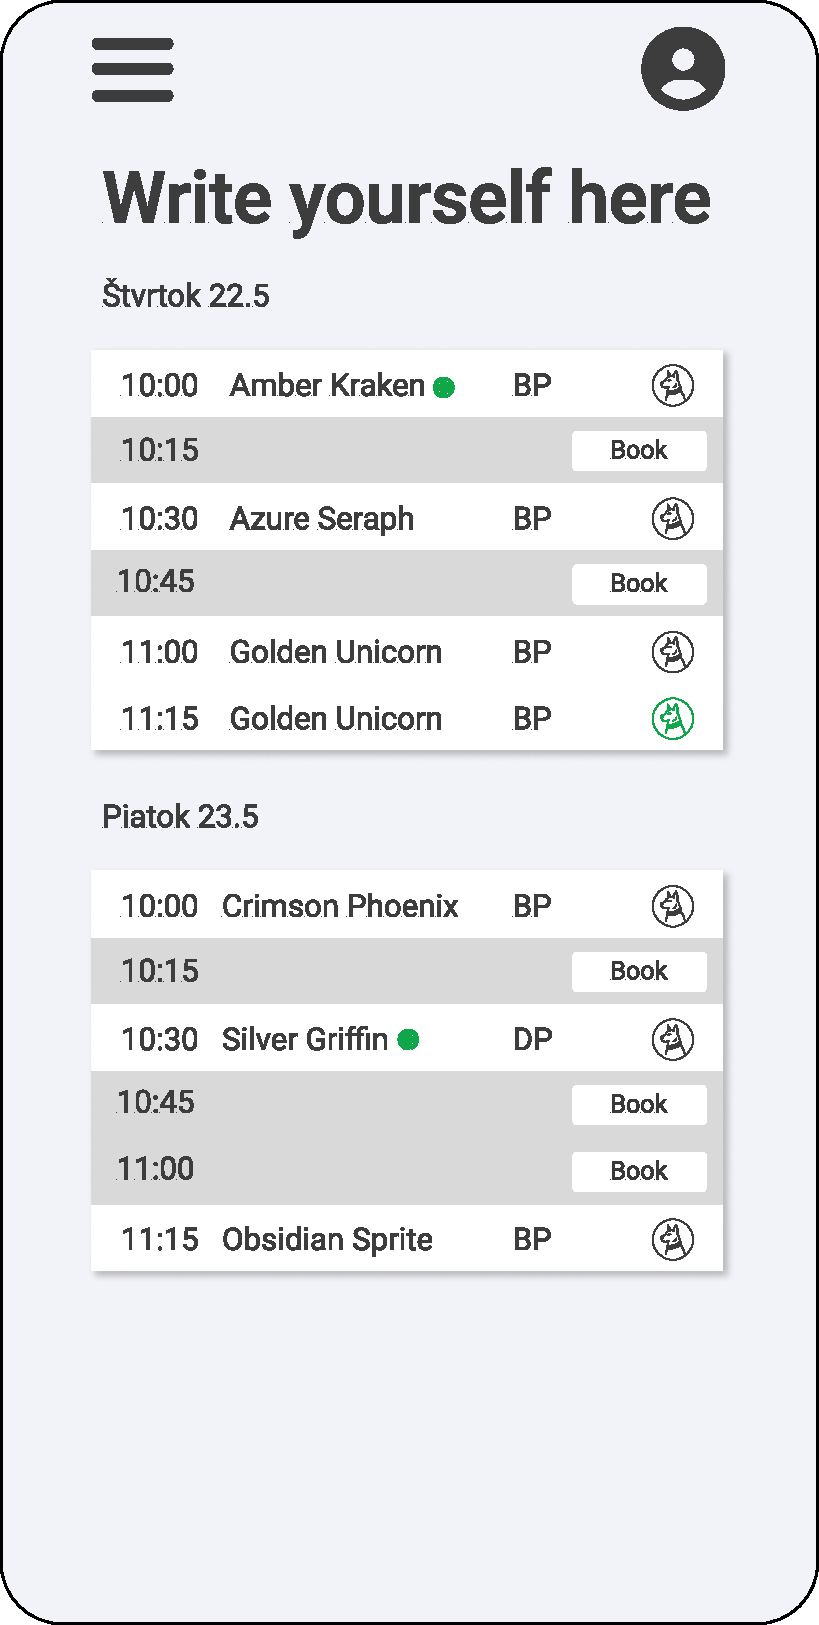
\includegraphics[width=\textwidth]{obrazky-figures/navrh-visitor-old.pdf}
        \caption{Prvý prototyp domovskej obrazovky Návštevníka s tlačidlami Book a ikonkami strážneho psa.}
        \label{fig:visitor-old}
    \end{minipage}
    \hfill
    \begin{minipage}[t]{0.45\textwidth}
        \centering
        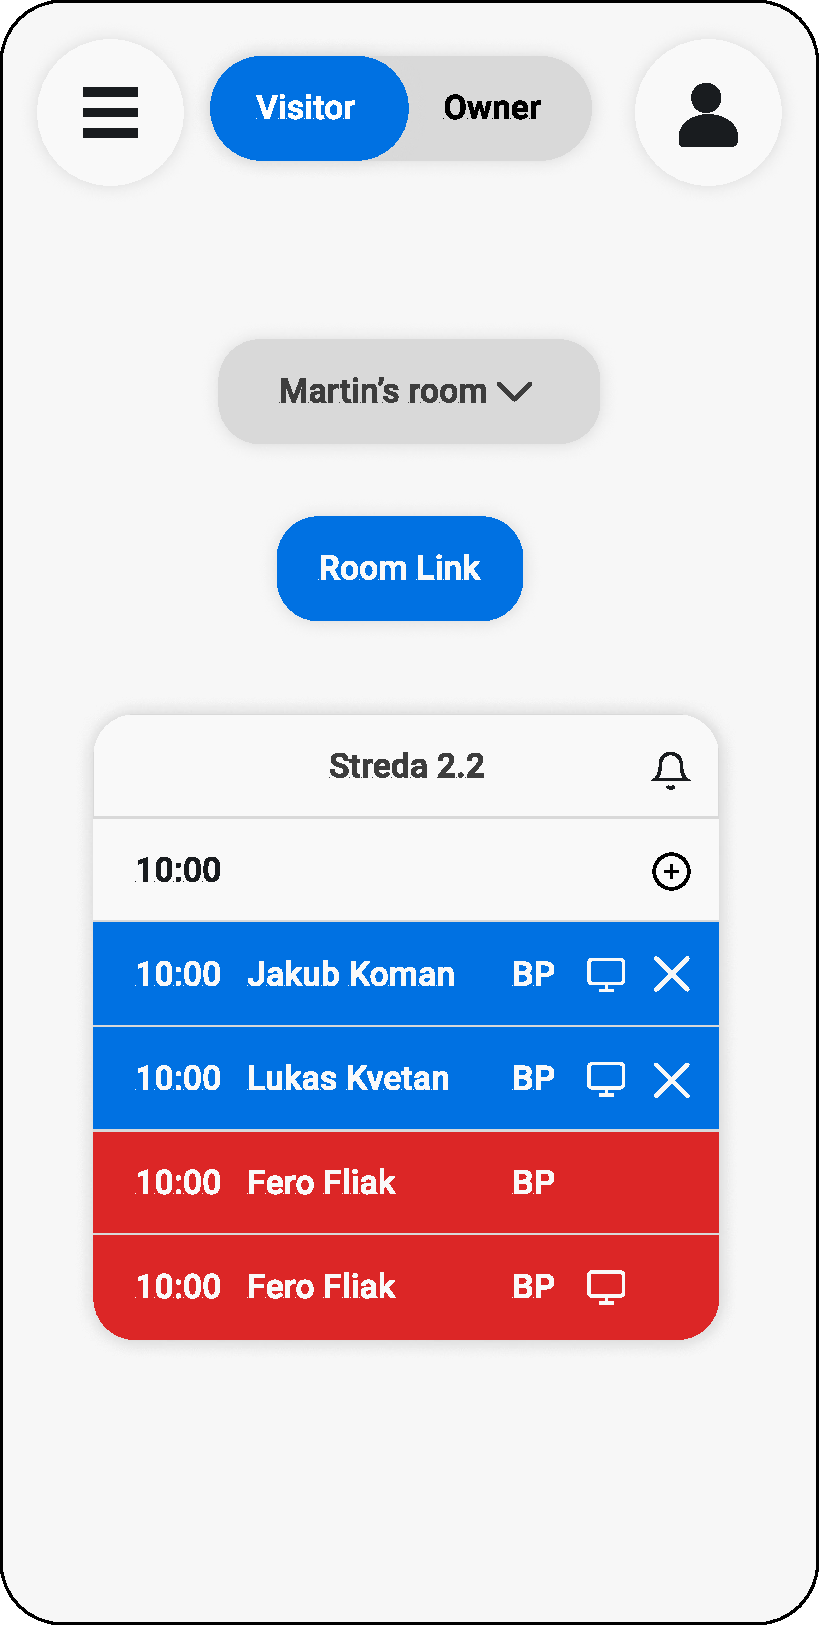
\includegraphics[width=\textwidth]{obrazky-figures/navrh-visitor.pdf}
        \caption{Druhý prototyp domovskej obrazovky Návštevníka po iteratívnych úpravách: odstránené tlačidlá Book, zjednodušené ikonky a pridaný prepínač medzi rolami.}
        \label{fig:visitor-new}
    \end{minipage}
\end{figure}

\subsection{Pohľad Majiteľa}
Majiteľ má nad hlavnou obrazovkou s miestnosťami umiestnený toggle, ktorý mu umožňuje 
kedykoľvek prepnúť sa do režimu Návštevníka – napríklad v prípade, ak sám potrebuje 
navštíviť konzultácie iného vyučujúceho. Toto riešenie priamo vychádza zo špecifikácie 
požiadaviek uvedenej v kapitole~\ref{chap:analyza}, kde jeden používateľ môže v rôznych 
miestnostiach vystupovať v oboch rolách súčasne.

Priamo pod prepínačom miestností a odkazovým tlačidlom miestnosti sa nachádza tlačidlo 
s ikonkou plus, ktoré slúži na rýchle vytvorenie nového bloku bez nutnosti prechádzať 
cez menu. Vedľa neho je umiestnená ikonka troch bodiek (\textit{3 dots}), ktorá po 
kliknutí zobrazí kontextové menu s možnosťami správy miestnosti: \textit{Edit Room}, 
\textit{Delete Room} a \textit{Show Users Joined} – prehľad Návštevníkov pripojených do miestnosti.

Majiteľ má na hlavnej obrazovke oproti Návštevníkovi rozšírené možnosti správy 
jednotlivých slotov. Pri každom slote je dostupná ikonka histórie, ktorej kliknutím 
sa zobrazí história daného slotu. Majiteľ má zároveň možnosť meniť stav slotu medzi 
online a offline režimom, a to aj pri slotoch, ktoré sú už rezervované Návštevníkom. 
Práve v takom prípade sú obzvlášť užitočné e-mailové notifikácie – ak Majiteľ zmení 
napríklad prezenčnú konzultáciu na online z dôvodu choroby, systém automaticky upozorní 
dotknutého Návštevníka e-mailom, pokiaľ má notifikácie povolené v nastaveniach.

Podobne ako pri obrazovke Návštevníka, aj pohľad Majiteľa prešiel iteratívnym vývojom. V prvom prototype (obrázok~\ref{fig:owner-old}) chýbali tlačidlá na správu miestnosti a bloku, ikonka plus na pridanie bloku bola umiestnená na spodku obrazovky a prekrývala sa s blokmi. Obsadené sloty boli rozlíšené len pomocou checkboxov bez farebného kódovania. Na základe spätnej väzby bol znova vytvorený druhý prototyp (obrázok~\ref{fig:owner-new}): ikonka plus bola presunutá priamo pod odkaz na miestnosť, boli pridané farebné stavy slotov, tlačidlo \textit{Edit Block} a menu pre správu miestnosti (\textit{Edit Room}, \textit{Delete Room}, \textit{Show Users Joined}).

\subsubsection*{Vytvorenie a editácia miestnosti}
Pri vytváraní miestnosti Majiteľ nastaví nasledujúce atribúty:
\begin{itemize}
    \item \textbf{Title:} Názov miestnosti (napríklad \textit{Martin's Room}).
    \item \textbf{Room description:} Popis miestnosti zobrazený Návštevníkom, napríklad číslo kancelárie na fakulte (\textit{L224}).
    \item \textbf{Link:} Externý odkaz priradený k miestnosti, napríklad link na online konzultácie alebo osobná webová stránka vyučujúceho.
    \item \textbf{Cancellation hours:} Počet hodín pred začiatkom konzultácie, do ktorých môže Návštevník zrušiť svoju rezerváciu bez varovania. Pri neskoršom zrušení systém zobrazí upozornenie, že toto konanie plytvá časom ostatných študentov aj vyučujúceho.
    \item \textbf{Allowed e–mails list:} Správa prístupu k miestnosti. Majiteľ môže povoliť prístup konkrétnym e-mailovým adresám alebo celým doménam. Zadaním požadovaného textu a následným kliknutím na potvrdzujúcu ikonku vpravo pridá Majiteľ tento text do zoznamu povolených e-mailov, ktorý sa dá zobraziť nižšie.
\end{itemize}
Obrazovka editácie miestnosti umožňuje úpravu všetkých vyššie uvedených atribútov. Majiteľ má zároveň k dispozícii možnosť zobraziť zoznam Návštevníkov pripojených do miestnosti, zobraziť históriu slotov a natrvalo vymazať miestnosť.

\subsubsection*{Vytvorenie a editácia bloku}
Pri vytváraní bloku Majiteľ najprv vyberie jeden alebo viacero dátumov. Výber podporuje dva režimy: výber jednotlivých dní (1-n nesúvisiacich dátumov) alebo výber súvislého časového rozsahu (\textit{range}). Vďaka tejto funkcii môže Majiteľ jednou akciou vytvoriť bloky na viacero dní naraz, čo výrazne znižuje administratívnu záťaž pri pravidelných konzultáciách. Následne nastaví ďalšie parametre bloku:
\begin{itemize}
    \item \textbf{Block start time:} Čas začiatku bloku, teda prvého slotu v bloku, nastaviteľný pomocou časového scrollera.
    \item \textbf{Minutes per slot:} Trvanie jedného slotu v minútach, volený taktiež pomocou časového scrollera.
    \item \textbf{Slot count:} Počet slotov, ktoré budú vytvorené.
    \item \textbf{Block end time:} Na základe zadaného počtu slotov, ich trvania a času začatia prvého slotu sa automaticky vypočíta čas ukončenia bloku (\textit{end time}).
    \item \textbf{Note:} Voliteľná textová poznámka pre Návštevníkov viditeľná v hlavičke bloku.
    \item \textbf{Is online:} Označenie bloku ako online konzultácie.
\end{itemize}

V obrazovke editácie bloku môže Majiteľ mazať jednotlivé sloty, prepínať blok a sloty medzi online a offline stavom, vymazať celý blok alebo ho nakopírovať na iný dátum. Pridanie nového slotu je možné tromi spôsobmi: kliknutím na tlačidlo plus pred prvým slotom v bloku, kliknutím na tlačidlo plus za posledným slotom v bloku, alebo presmerovaním z obrazovky editácie bloku na obrazovku pridania slotu s možnosťou zadania konkrétneho požadovaného času.
\begin{figure}[t]
    \centering
    \begin{minipage}[t]{0.45\textwidth}
        \centering
        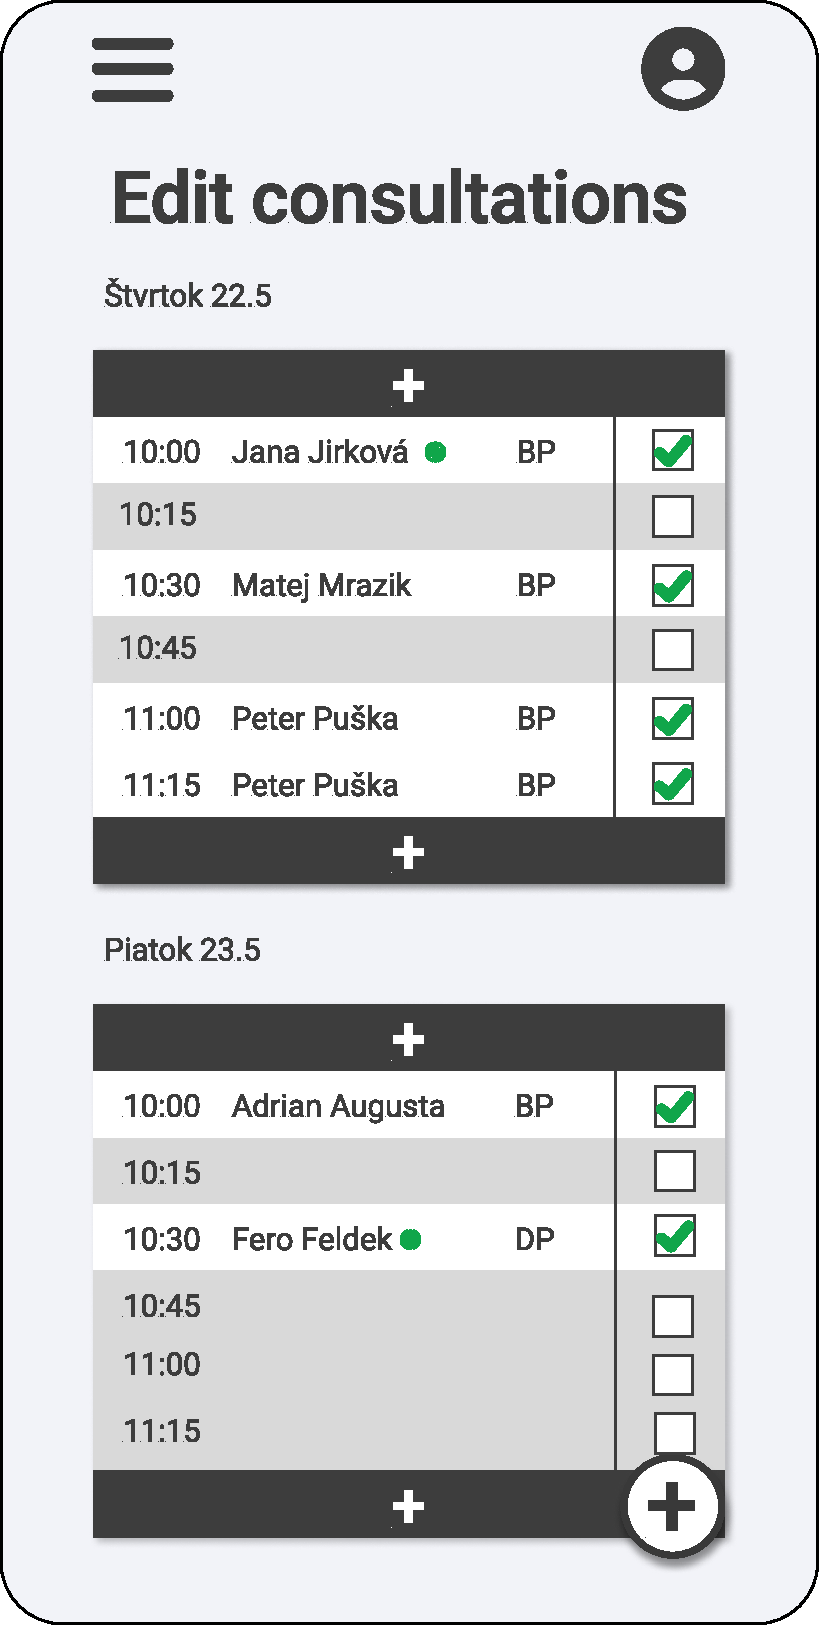
\includegraphics[width=\textwidth]{obrazky-figures/navrh-owner-old.pdf}
        \caption{Prvý prototyp domovskej obrazovky Majiteľa s checkboxmi a bez tlačidiel na správu.}
        \label{fig:owner-old}
    \end{minipage}
    \hfill
    \begin{minipage}[t]{0.45\textwidth}
        \centering
        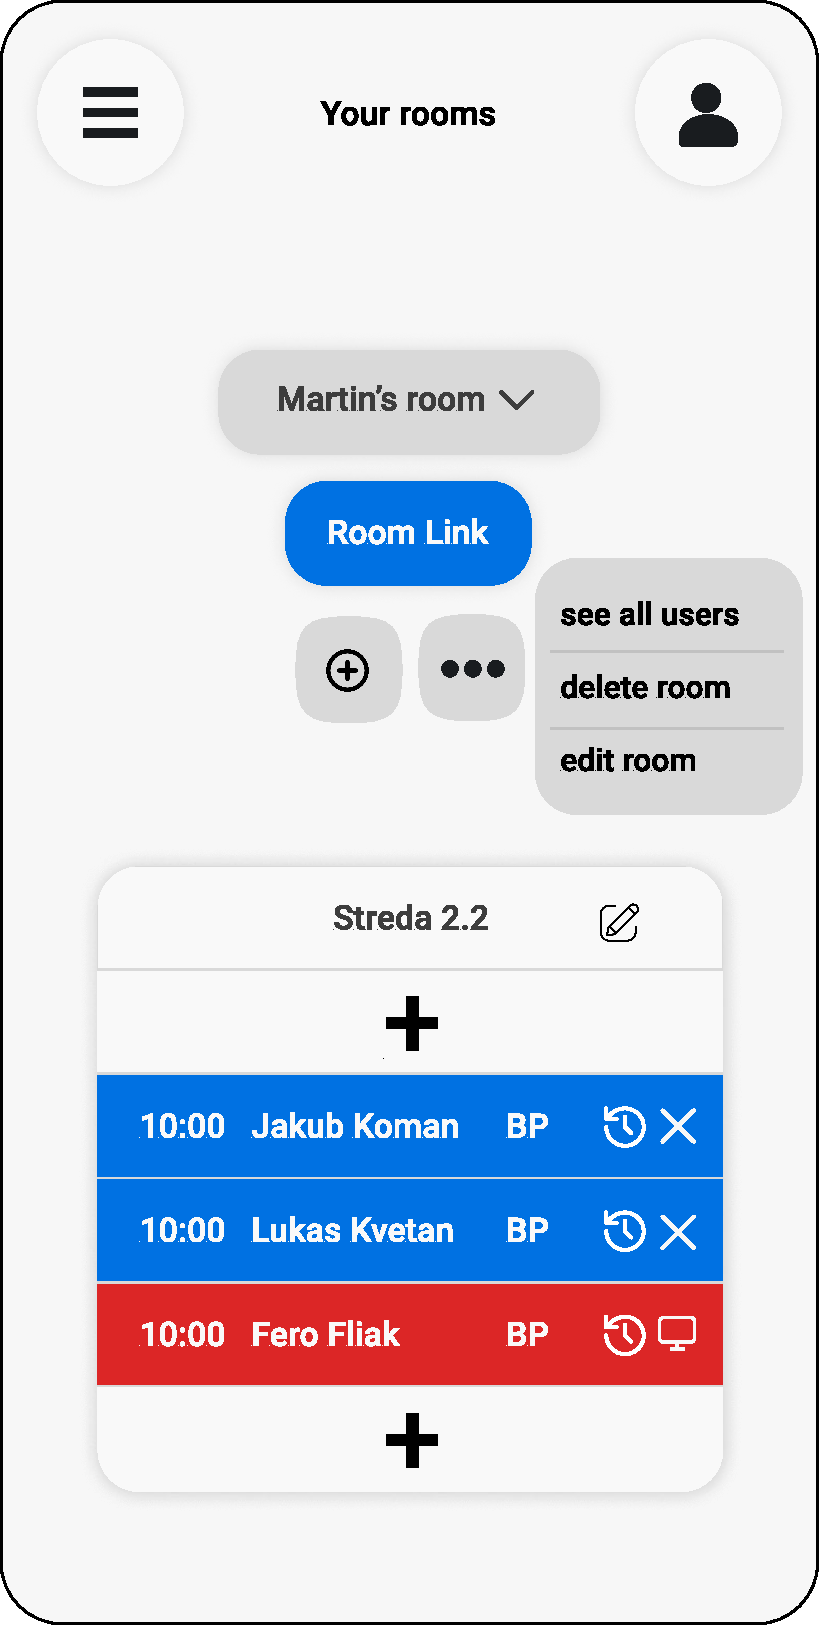
\includegraphics[width=\textwidth]{obrazky-figures/navrh-owner-new.pdf}
        \caption{Druhý prototyp domovskej obrazovky Majiteľa s farebnými slotmi, presunutým tlačidlom plus a pridanými nástrojmi na správu bloku a miestnosti.}
        \label{fig:owner-new}
    \end{minipage}
\end{figure}


\begin{figure}[t]
    \centering
    \begin{minipage}[t]{0.45\textwidth}
        \centering
        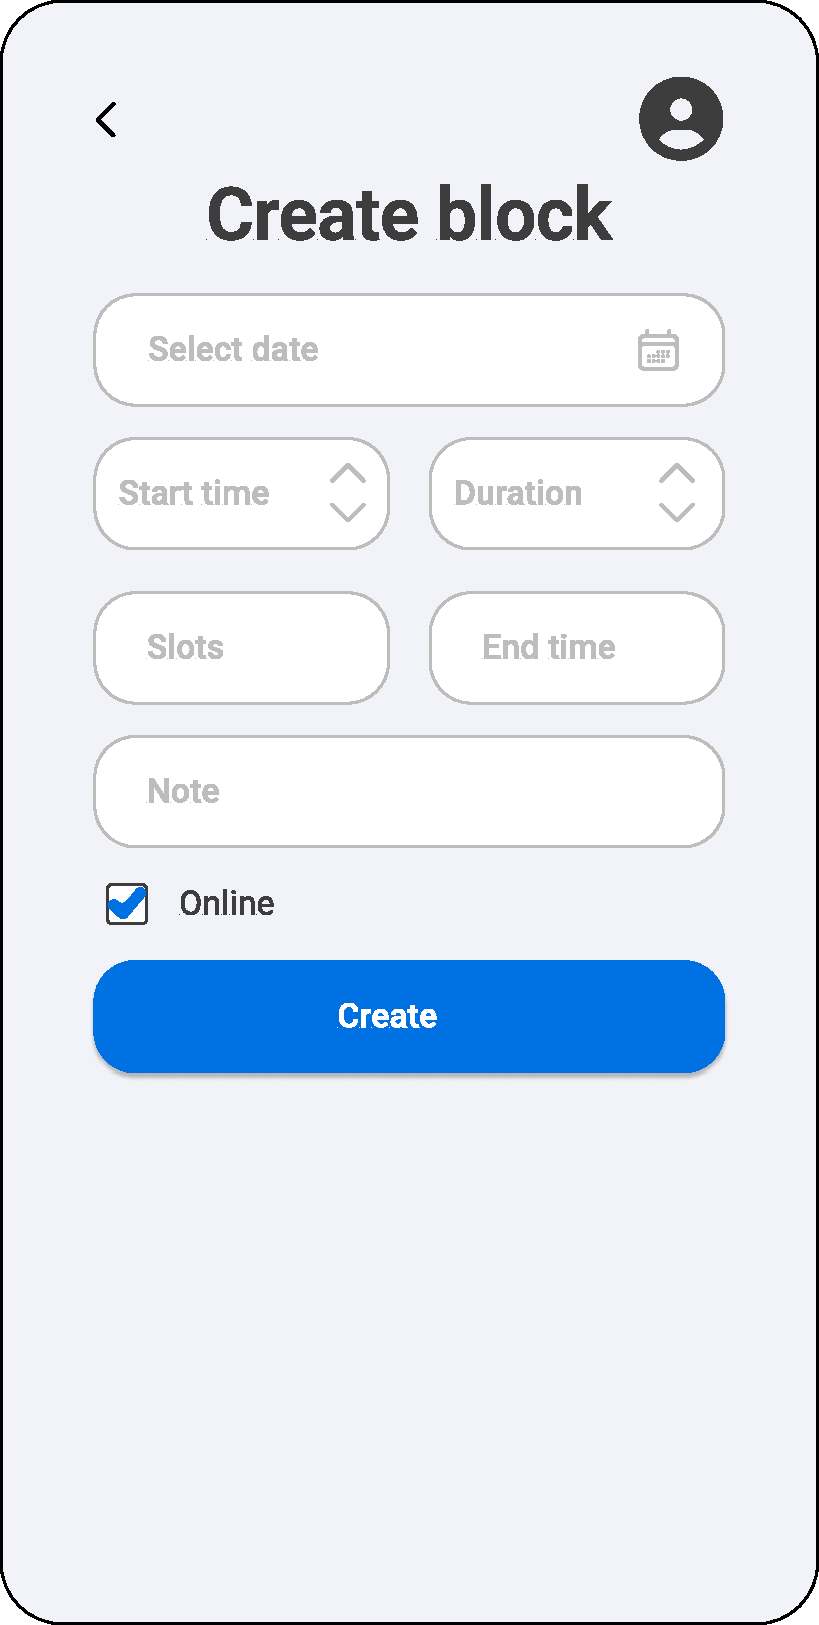
\includegraphics[width=\textwidth]{obrazky-figures/navrh-create-block.pdf}
       
    \end{minipage}
    \hfill
    \begin{minipage}[t]{0.45\textwidth}
        \centering
        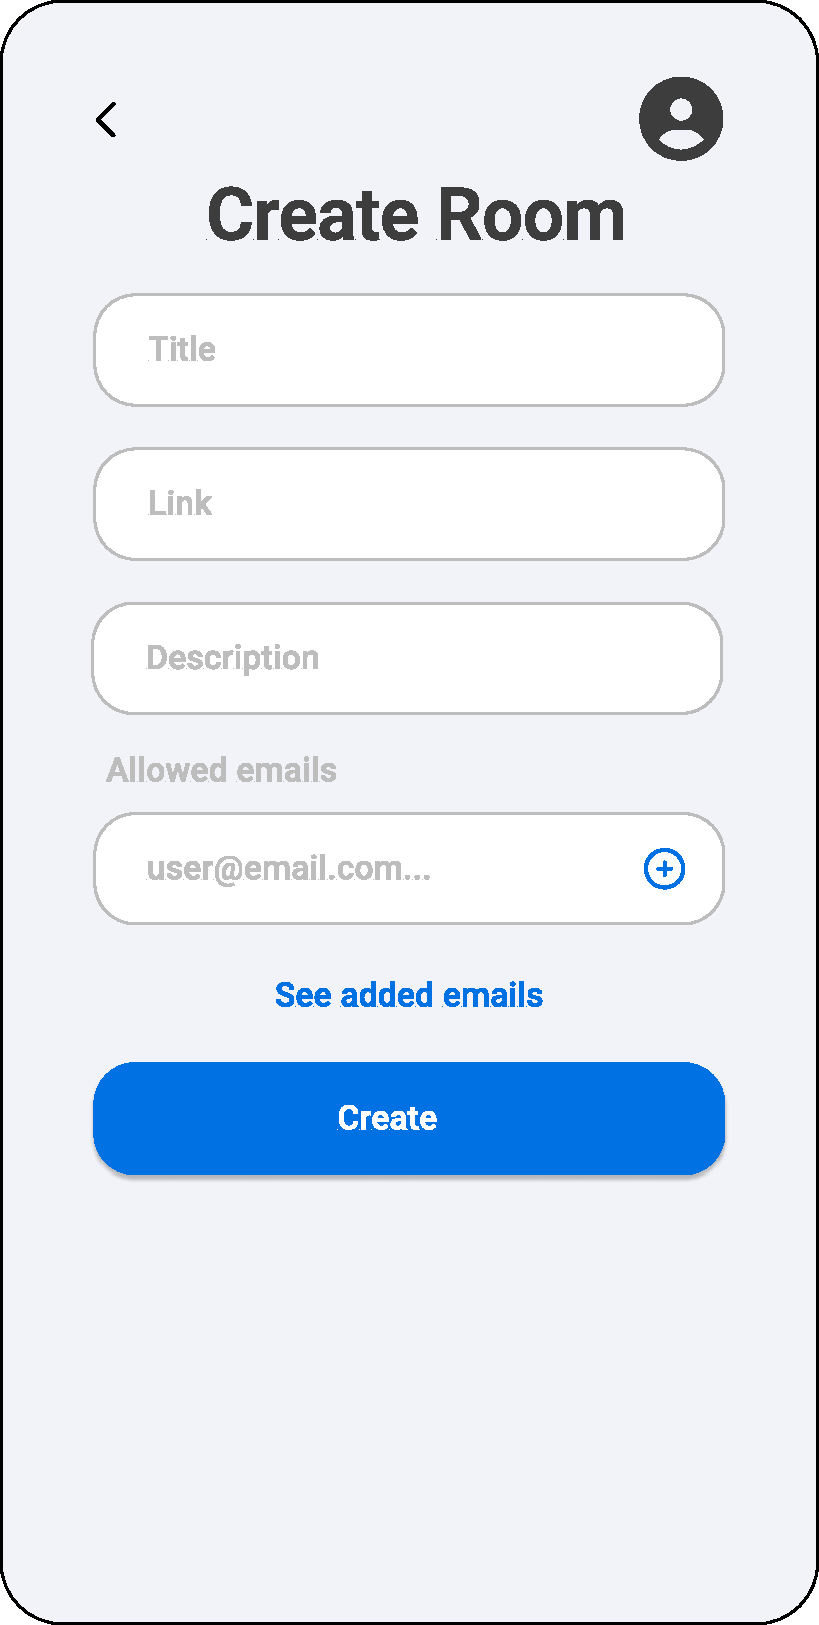
\includegraphics[width=\textwidth]{obrazky-figures/navrh-create-room.pdf}
       
    \end{minipage}
     \caption{Prototypy obrazoviek na vytvorenie bloku (naľavo) a miestnosti s možnosťou dynamického pridávania e-mailov (napravo).}
    \label{fig:create-block-room}
\end{figure}

\subsection{Navigácia a nastavenia}

\subsubsection*{Hamburger menu a možnosť návratu}
Bočné vysúvacie menu je prístupné výlučne z hlavnej obrazovky (\textit{home screen}) 
prostredníctvom ikony v ľavom hornom rohu. Na všetkých ostatných obrazovkách 
je namiesto neho zobrazená šípka späť, ktorá používateľa vráti o úroveň vyššie. 
Keďže aplikácia nie je hlboko vnorená, niekoľkými krokmi späť sa používateľ 
vždy rýchlo dostane na hlavnú obrazovku, odkiaľ má opäť prístup k menu. 
Toto riešenie vychádza z heuristiky kontroly a slobody používateľa popísanej 
v sekcii~\ref{sec:navrh-ui} – používateľ má vždy k dispozícii jasný 
a predvídateľný spôsob návratu. Menu obsahuje nasledujúce položky: 
\textit{Home}, \textit{Join Room}, \textit{Create Room} (len Majiteľ), \textit{Provide Feedback} 
a \textit{Settings}. Položka \textit{Logout} je zámerne zvýraznená červenou 
farbou ako deštruktívna akcia, čím sa predchádza náhodnému odhláseniu.

\subsubsection*{Nastavenia a správa profilu}
Obrazovka nastavení (obrázok~\ref{fig:settings}) je dostupná obom rolám a obsahuje nasledujúce možnosti:
\begin{itemize}
    \item \textbf{Edit profile:} Úprava mena, priezviska a dôvodu návštevy, ktorý sa Majiteľovi zobrazuje pri rezervovaných slotoch.
    \item \textbf{Visibility:} Možnosť skryť vlastné meno voči ostatným používateľom z dôvodov ochrany osobných údajov (GDPR). Ako prirodzený dôsledok tohto nastavenia používateľ sám neuvidí mená ostatných.
    \item \textbf{Notify me before:} Nastavenie e-mailových notifikácií pred začiatkom konzultácie. Určuje počet hodín pred začiatkom konzultácie, kedy má byť upozornenie odoslané.
    \item \textbf{Theme:} Prepínač vizuálneho motívu aplikácie.
    \item \textbf{Create Teacher:} Funkcia dostupná výlučne pre Majiteľa, ktorá umožňuje udeliť rolu Majiteľa inému používateľovi.
\end{itemize}

\begin{figure}[t]
    \centering
    \begin{minipage}[t]{0.45\textwidth}
        \centering
        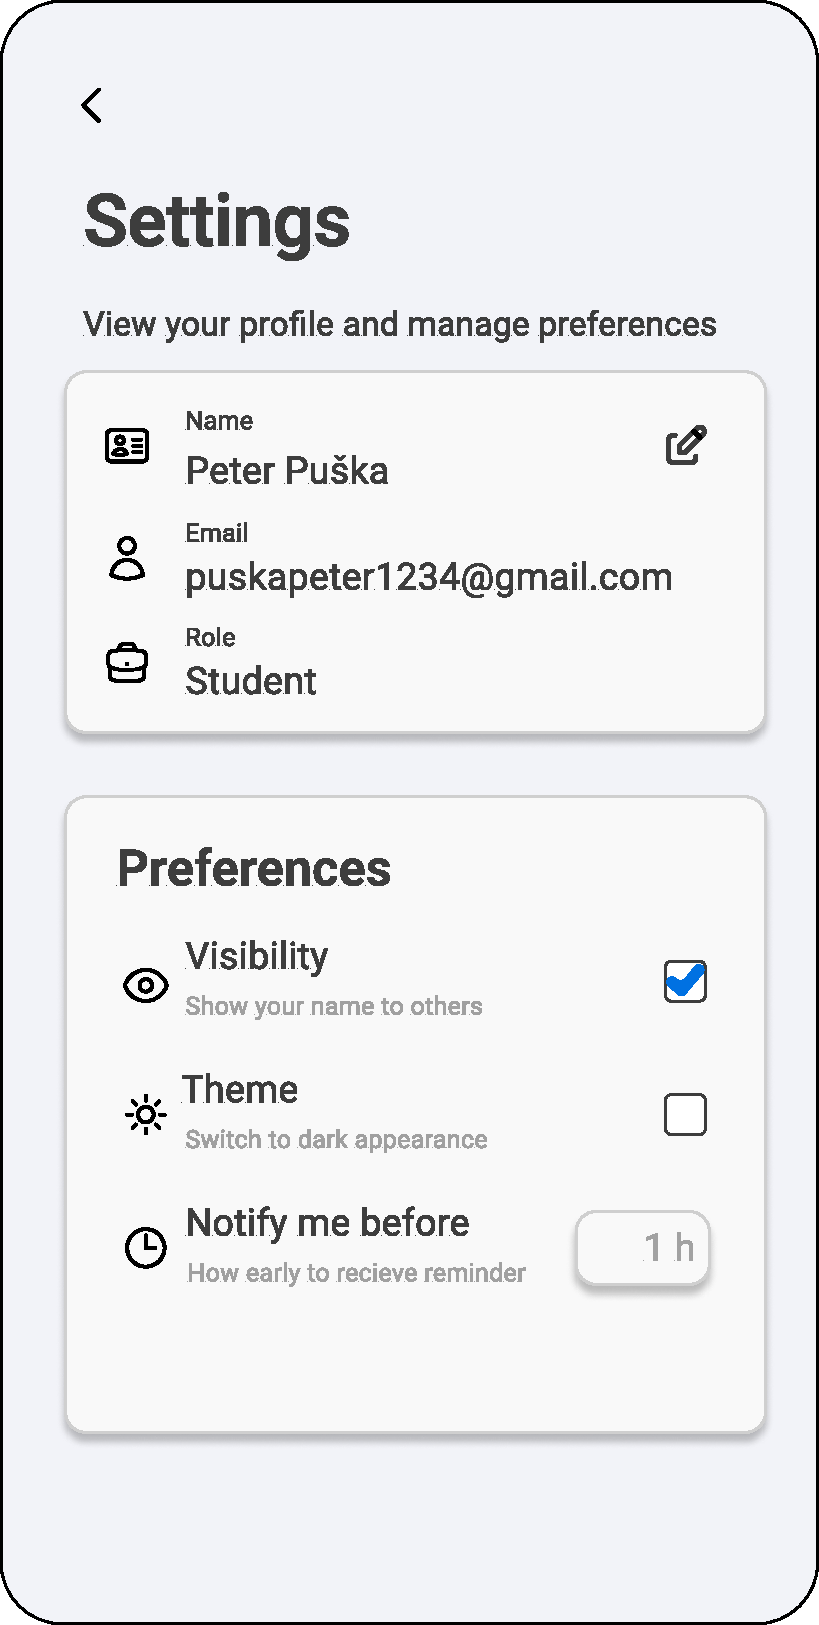
\includegraphics[width=\textwidth]{obrazky-figures/navrh-settings.pdf}
        \caption{Prototyp znázorňujúci obrazovku nastavení Návštevníka. Majiteľ by mal možnosť navyše vytvoriť nového učiteľa.}
        \label{fig:settings}
    \end{minipage}
    \hfill
    \begin{minipage}[t]{0.45\textwidth}
        \centering
        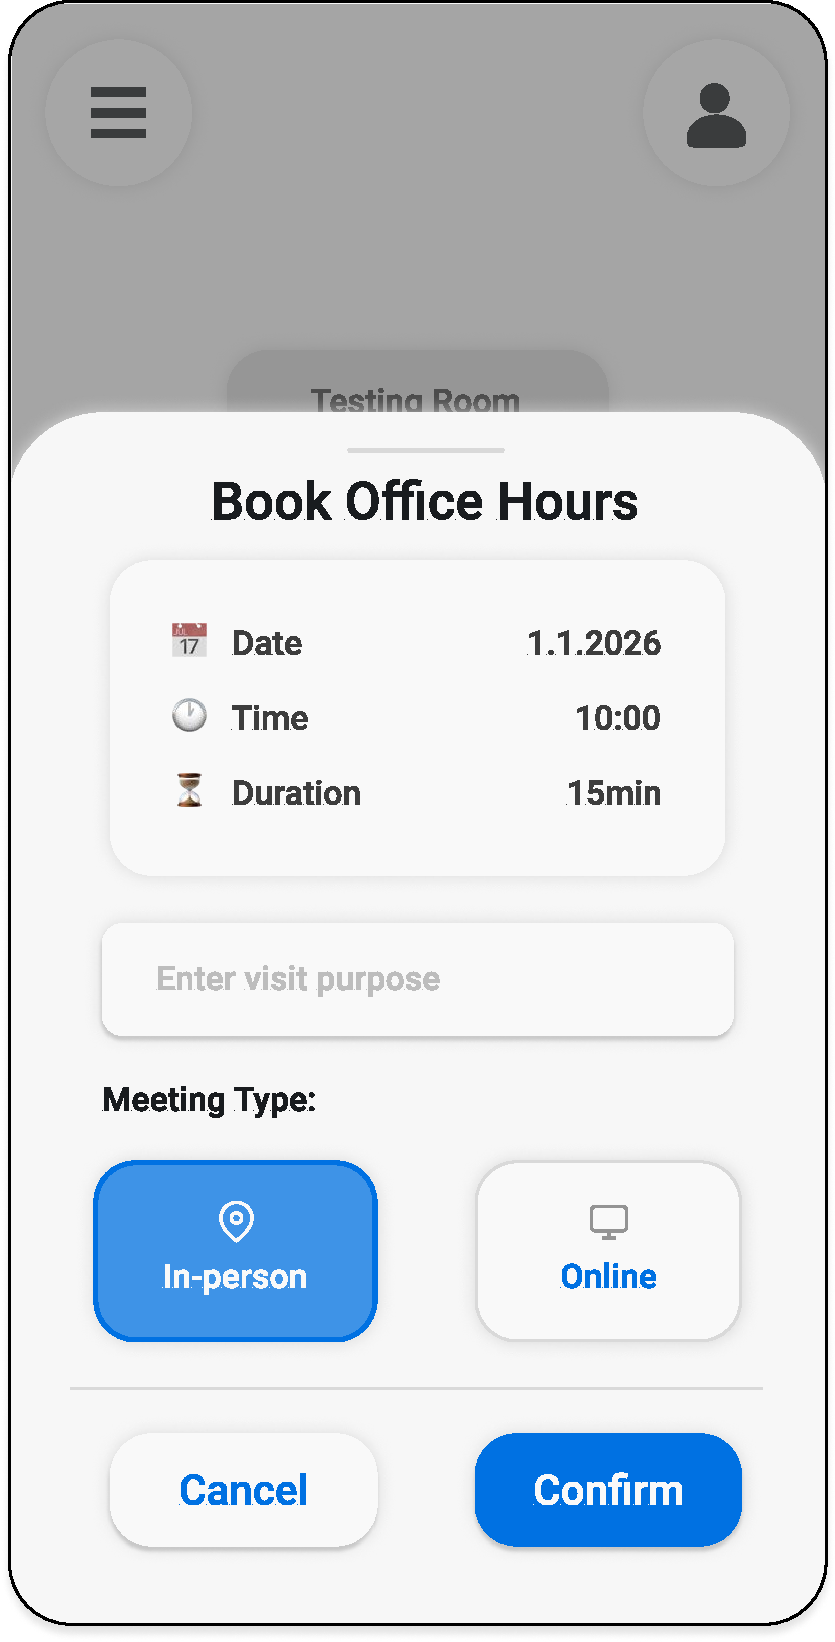
\includegraphics[width=\textwidth]{obrazky-figures/navrh-slot-taking.pdf}
        \caption{Prototyp znázorňujúci dialóg na rezervovanie slotu s dôvodom návštevy a prepínačom online/offline.}
        \label{fig:slot-dialog}
    \end{minipage}
\end{figure}

\section{Návrh softvérovej architektúry}
Aby bol zdrojový kód udržateľný, testovateľný a pripravený na budúce rozširovanie, bolo kľúčové zvoliť vhodnú softvérovú architektúru, ktorá striktne oddeľuje používateľské rozhranie od biznis logiky. Výber architektonického vzoru MVVM a jeho teoretické porovnanie s vzormi MVC a MVP je podrobne zdôvodnené v kapitole~\ref{sec:architektura-mvvm}.

\subsection{Adresárová štruktúra a pomenovacie konvencie}
\label{subsec:strukturanavrh}
Pre zabezpečenie dlhodobej udržateľnosti kódu, vysokej čitateľnosti a jednoduchej orientácie v projekte pre prípadných ďalších vývojárov, boli už vo fáze návrhu definované striktné pravidlá pre organizáciu súborov a pomenovacie konvencie (Naming Conventions). Projekt Office Hours sa pri ich definovaní riadil oficiálnymi odporúčaniami jazyka Dart známymi ako \textit{Effective Dart Guidelines}~\cite{effectivedart}:
\begin{itemize}
    \item \textbf{Triedy, modely a enumeračné typy:} Využívajú formát \textbf{UpperCamelCase} (tiež známy ako PascalCase). Každé slovo v názve vrátane prvého začína veľkým písmenom bez akýchkoľvek oddeľovacích znakov. Príklad: \textbf{CreateBlockViewModel} alebo \textbf{ApiService}.
    \item \textbf{Premenné, konštanty a inštancie objektov:} Využívajú formát \textbf{camelCase}. Prvé slovo začína malým písmenom a každé ďalšie veľkým. Príklad: \textbf{selectedRoomId} alebo \textbf{isTeacher}.
    \item \textbf{Súbory a adresáre:} Pre názvy samotných súborov v súborovom systéme bol striktne zvolený formát \textbf{snake\_case}, kde sú všetky písmená malé a slová sú oddelené podčiarkovníkom. Príklad: \textbf{create\_block\_viewmodel.dart}.
\end{itemize}

Samotná logická adresárová štruktúra projektu (nachádzajúca sa v primárnom koreňovom priečinku \textbf{lib/}) bola priamo odvodená od zvolenej architektúry MVVM. Rozdelenie do logických modulov zaručuje, že vývojár vždy presne vie, kam má umiestniť nový kód:
\begin{itemize}
    \item \textbf{models/}: Priečinok obsahujúci všetky dátové triedy slúžiace na mapovanie JSON odpovedí zo servera do vnútorných štruktúr jazyka Dart.
    \item \textbf{views/}: Priečinok obsahujúci výlučne prezentačnú vrstvu aplikácie. Nachádzajú sa tu jednotlivé samostatné obrazovky (Pages) a podpriečinok \textbf{custom\_widgets/}, v ktorom sú uložené znovupoužiteľné vizuálne komponenty.
    \item \textbf{viewmodels/}: Každá komplexná obrazovka má tu svoj zodpovedajúci \textbf{ViewModel}, ktorý pre ňu spravuje stav a komunikuje so sieťovou vrstvou.
    \item \textbf{services/}: Priečinok združujúci rozličné služby. Obsahuje \textbf{api\_service.dart} pre sieťovú komunikáciu, \textbf{user\_preferences.dart} pre prístup k lokálnemu úložisku a taktiež súbory pre centrálnu správu navigácie, akými sú \textbf{app\_router.dart} a služby navigátora, ktoré riadia smerovanie a plynulé prechody medzi jednotlivými obrazovkami aplikácie.
    \item \textbf{utils/}: Zložka vyhradená pre statické pomocné triedy, definície globálnych konštánt (\textbf{constants.dart}) a validátory používateľských vstupov.
\end{itemize}

\section{Možnosti rozšírenia}
Architektúra aplikácie Office Hours bola od počiatku navrhovaná s ohľadom na dlhodobú udržateľnosť a prípadné predanie kódu ďalej budúcim vývojárom.

\subsection{Pripravenosť na platformu iOS}
Jedným z hlavných dôvodov pre výber frameworku Flutter bola jeho schopnosť kompilovať jedinú spoločnú bázu kódu do natívnych aplikácií pre viaceré operačné systémy. Vzhľadom na hardvérové obmedzenia počas tvorby tejto práce (absencia platformy macOS potrebnej pre kompiláciu cez vývojové prostredie Xcode) bola aplikácia nasadená, testovaná a publikovaná primárne pre platformu Android.

Zdrojový kód je pripravený aj na bežanie v operačnom systéme iOS a budúci vývojár môže tento existujúci kód s minimálnymi úpravami publikovať priamo do obchodu App Store. Tento prístup šetrí potenciálnym budúcim vývojárom hodiny času, ktoré by inak boli potrebné na vývoj samostatnej aplikácie napríklad v jazyku Swift.

\subsection{Ďalšie rozšírenia}
Možným rozšírením by bola integrácia \textbf{push notifikácií}, ktorá by aktívne upozornila študenta na blížiaci sa rezervovaný termín alebo na jeho zrušenie učiteľom. Prínosná by bola aj \textbf{integrácia s kalendárom} zariadenia, kde by aplikácia po potvrdení rezervácie automaticky vytvorila udalosť vrátane polohy miestnosti, čím by sa eliminovalo riziko zabudnutia termínu. \textbf{Offline režim} s lokálnou vyrovnávacou pamäťou by zase umožnil zobrazenie naposledy načítaných dát aj bez aktívneho internetového pripojenia.

Ďalším prínosom by bola \textbf{integrácia s aplikáciou VUT}, ktorá by umožnila zobrazovať potvrdené rezervácie priamo v rozvrhu študenta vedľa bežných predmetov, čím by vznikol jednotný prehľad akademických povinností na jednom mieste. Užitočným doplnkom by bola aj podpora \textbf{profilovej fotografie} používateľa, ktorá by učiteľovi uľahčila identifikáciu študentov v zozname rezervácií. V neposlednom rade by \textbf{mesačný prehľad rezervácií v kalendári} vizuálne zvýraznil dni s aktívnou rezerváciou, čo by používateľovi umožnilo okamžitú orientáciu v jeho rezerváciách.